% HTTP (Hypertext Transfer Protocol)
% - Übertragung von Web-Inhalten (Daten für websites)
% - Client-Server-Kommunikation: Clients fragen Webinhalte von Servern an
% - Request-Response Pattern
% - Stateless: Request-Response unabhängig, Kommunikation nicht wiederaufnehmbar
%
% Erweiterungen seit Version 2
% - Multiplexing and Stream Prioritization: 
%     - Mehrere Anfragen und Antworten gleichzeitig
%     - TCP Erweiterung
%     - blocking
% - Push Benachrichtigung:
%     -  Server mehrere Responses auf eine Anfrage
%     - Verbindungen werden nicht sofort geschlossen
% - QUIC 
%     - transport layer Protokoll
%     - nicht mehr TCP basiert
% 
% **Für WAF HTTP v1 Relevant**
% - Grundlegendes HTTP schema verstehen
% 
% **Protokoll**
% Kommunikationsprozess:
% 1. Verbindungsaufbau
%     - Client -> Server
% 2. Anfrage 
%     - Client fragt Daten an oder löst Aktion aus
% 3. Antwort 
%     - Server quittiert Anfrage
%     - eventuell Daten als Antwort
% 4. Verbindung schließen
%     - Server kann eigenständig keine Verbindung zu client mehr herstellen
% 
% Kommunikationsschema:
% 
% HTTP-Request
% - Startzeile:
%     - Methode: 
%         - Aktion (GET, POST, ...)
%         - angelehnt an SQL Datenbank Operationen
%     - Anfrage-URL
%         - Pfad entsprechen UNIX-Path
%         - Prameter (filter) nach `?`
%     - HTTP-Version: 
%         - Version der folgenden Kommunikation
% - Header
% - Body
% 
% HTTP-Response
% - Statuszeile:
%     - Status Code: 
%         - Numerischer Code
%         - Status der Verarbeitung (200:OK, 400 User Fehler, 500: Server Fehler, ...)
%     - Status-Text: 
%         - Beschreibung des Status code
% - Header
% - Body
% 
% HTTP-Header:
% - zusätzliche Informationen (Host, User-Agent, Content-Type, ..)
% - Enthalten Metadaten über die Anfrage oder den Client/Server.
% 
% HTTP-Body
% - Optional
% - Daten

Das Hypertext Transfer Protokoll (HTTP) ist ein Protokoll in der Internet-Kommunikation, dass zur übertagung diverser Daten unterschiedlicher Datentypen genutzt werden kann. Sein Haupt-Einsatzgebiet ist die Datenübertragung zwischen Webseiten und Clients.
Seit der Einführung in 1991 wurde es in mehreren RFCs erweitert und ist inzwischen in version drei.\\

In seiner aktuellen Form kann es Gebrauch von TCP-Sitzungen machen um Verbindungen über längere Zeit aufrecht zu halten und fortgeschrittenere Kommunikation, wie push Nachrichten, zu erlauben. Außerdem kann TCP-Pipelining genutzt werden um die parallele Abarbeitung von Anfragen zu ermöglichen und nicht auf die \textit{Acknowledge}-Nachrichten von TCP warten zu müssen.
Um seine Grundfunktion zu erläutern wird in diesem Kapitel die statuslose Kommunikation, definiert in Version 1.0 die mit einem unmittelbaren Anfrage-Antwort Muster arbeitet, beschrieben.
Hierin initiiert ein Client mit einer Anfrage Nachricht \footnote{Im folgenden werden HTTP-Anfrage und das Englische HTTP-request synonym verwendet} eine Verbindung, die von einem Server verarbeitet und mit einer Antwort-Nachricht beantwortet wird. Darauf wird die Verbindung geschlossen.
Dem Sever ist es nun nicht mehr möglich dem Client weitere Daten zu senden, ohne das der Client eine weitere Anfrage-Nachricht schickt.

\paragraph{HTTP-Nachrichten}
Die Grundlegende Einheit einer \ac{http}-Kommunikation wird als \textit{Nachricht} bezeichnet.
Da \ac{http} ein Klartext-Protokoll ist, werden diese in menschenlesbarer Form als Text übertragen.
Eine Nachricht besteht aus einer \textit{Start-Zeile}, die die Nachricht entweder als Anfrage oder Antwort identifiziert. In diesen beiden Fällen hat die Zeile jeweils einen untersiedlichen Aufbau:

\begin{figure}[!hbt]
     \centering
     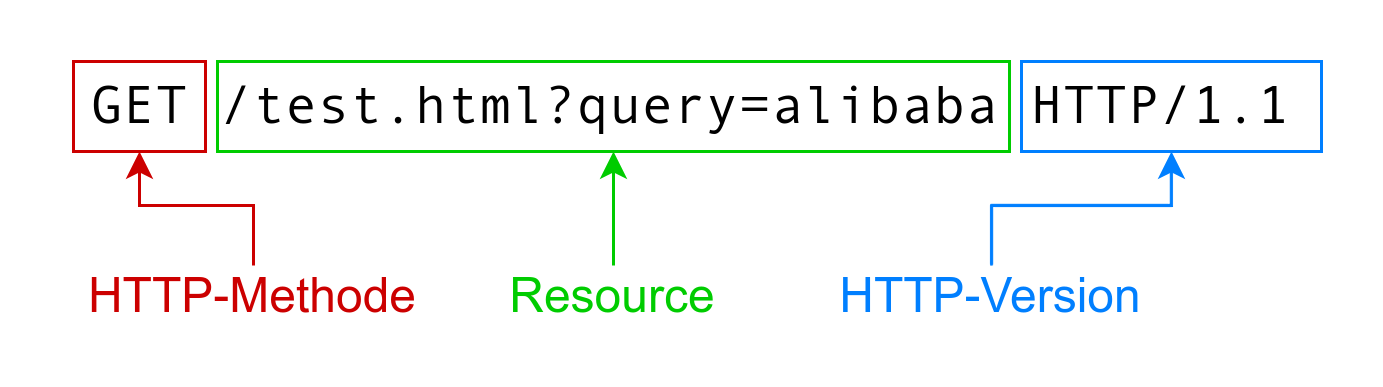
\includegraphics[width=0.9\textwidth]{./images/HTTP-Requestline.png}
     \caption{Beispiel für eine HTTP Request Zeile}
     \label{fig:http-requestline}
 \end{figure}

\begin{description}
     \item[Request-Zeile:] Ein HTTP-Request ist durch eine \textit{Request-Zeile} identifiziert. Diese ist in drei Teile Aufgeteilt (siehe Abb. \ref{fig:http-requestline}).
     \begin{description}
          \item[Die HTTP-Methode] beschreibt die Operation, die der Server ausführen soll und können auch \textit{HTTP-Verb} und \textit{HTTP-Noun} genannt werden.
          Syntaktisch basieren die Methoden auf dem FTP Protokoll, das älter ist und mit Operationen wie GET und PUT arbeitet.
          Der Satz an Verben und Nomen ist im Verlauf der HTTP Versionen jedoch um weitere Methoden, wie zum Beispiel PATCH oder OPTIONS, erweitert.
          \item[Die angefragte Resource] spezifiziert welche Resource angefragt wird. Üblicherweise eine URL. Optional kann die angefragte Resource mit einem Fragezeichen Gefolgt von einem sogenannten \textit{query string} noch spezifiziert beziehungsweise gefiltert werden.
          \item[Der HTTP Verion] die angibt in welcher Version die folgende Nachricht verfasst ist. 
     \end{description}
\end{description}

\begin{figure}[!hbt]
     \centering
     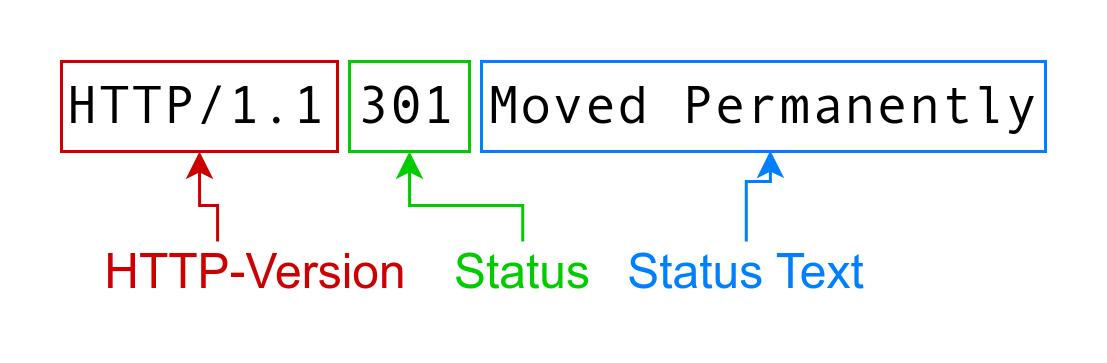
\includegraphics[width=0.9\textwidth]{./images/HTTP-Statusline.png}
     \caption{Beispiel für eine HTTP Status Zeile}
     \label{fig:http-statusline}
 \end{figure}


\begin{description}
     \item[Status-Zeile:] Die Antwort auf einen Request beginnt mit einer Status Zeile in einem eigenen Format, die wie die Request-Zeile aus drei Teilen besteht (siehe Abb. \ref{fig:http-statusline}).
     \begin{description}
          \item[Die HTTP Verion] gibt, wie an dritter Stelle des HTTP-Requests, die HTTP-Version der Folgenden Nachricht an.
          \item[Der Status code] der durch eine dreistellige Zahl angibt wie der Status der Verarbeitung eines Requests war. 
          Für verschiedene Ergebnisse ist ein Zahlenraum vorgeschrieben. 
          So steht zum Beispiel 2xx für eine Erfolgreiche Verarbeitung während 4xx auf einen Fehler auf Client-Seite hindeutet.
          \item[Der Status Text], einem Beliebigen den Text der den Status genauer beschreiben kann.
          Im HTTP Standard ist zwar nicht vorgeschrieben wie der Text auszusehen hat, es gibt jedoch Konventionen.
     \end{description}
\end{description}

Nach des Start Zeile folgen sowohl in einem HTTP-Request als auch in der Response zwei weitere Abschnitte. Diese werden genutzt um weitere Informationen an die Nachricht anzuhängen.

Die \textbf{HTTP-Header} sind Key-Value Pare. Der Key ist ein \textit{case sensitiver} String.
Der Value ist beliebig darf jedoch keinen Zeilenumbruch enthalten, da dies den Beginn eines neuen Header Key-Value-Pares anzeigt.
Die Header haben mehr unterkategorien wie \textit{Request-} oder \textit{General-Header}, hier ist es im Rahmen der Thesis jedoch nicht notwendig weiter in die Tiefe zu gehen.
Eine Relevante Header-Gruppe sine die \textit{Representation-Header} die die Formatierung des HTTP-Bodies genauer spezifizieren.
Hier kann der Datentyp und die Endcodierung des Bodies angegeben werden.

Der \textbf{HTTP-Body} enthält die Daten die mit der HTTP-Nachricht versendet werden. 
Er ist Optional.
Im Body können sich beliebige Daten befinden: Binärdaten wie Bilder, JSON-Formatierte String oder einfacher Text.\\

Wie man oben beschrieben sehen kann bietet HTTP eine Reichweite an Möglichkeiten an, einem Server Daten zu übergeben oder von einem solchen Daten zu erhalten.
Alle Felder werden verarbeitet und bieten somit Theoretisch die Möglichkeit zur Übermittlung schadhafter Daten genutzt zu werden.
Auch die Möglichkeit Daten zu Codieren, speziell im \textit{HTTP-Body}, kann zu diversen schadhaften Datenübertragungen führen.
Eine \ac{waf} muss in der Lage sein alle dieser Parameter Überblicken zu können um effektiven Schutz zu bieten.

\pagebreak    